In summer 2008 Daniel participated in the NSF-EAPSI (East Asian and Pacific Summer Institute) allowing him to study at the Hubo-Lab at KAIST to learn how to maintain, operate and program the Hubo series robot.
In Fall of 2008 Daniel started his work on a Hubo KHR-4 model in the Drexel Autonomous Systems Lab (DASL) at Drexel University.
Shortly after that in Spring of 2009 he had the robot performing interactive musical tasks such as listening to music and autonomously tapping its hand to the beat\cite{5686847}.
This was the first of many experiments in sensor integration on the Hubo.
Later that spring Daniel and the rest of DASL showed Hubo to the public at a live demonstration at the Philadelphia Please Touch Museum. 
In winter of 2009 the first of the visual feedback methods was implemented \cite{lofaroGamesRobot}.
In 2010 Daniel investigated brain machine interfacing with the robot as well as multi-modal sensing using visual and auditory cues\cite{lofaroIASTED2011}.
In late 2010/early 2011 Daniel started on his first throwing experiments which culminated in making the Hubo robot throw the first pitch at a Major League Baseball game\cite{lofaroHumanoids2012}.  
A timeline of Daniel's work can be seen in Fig.~\ref{fig:timeline}.

\begin{figure}[thpb]
  \centering
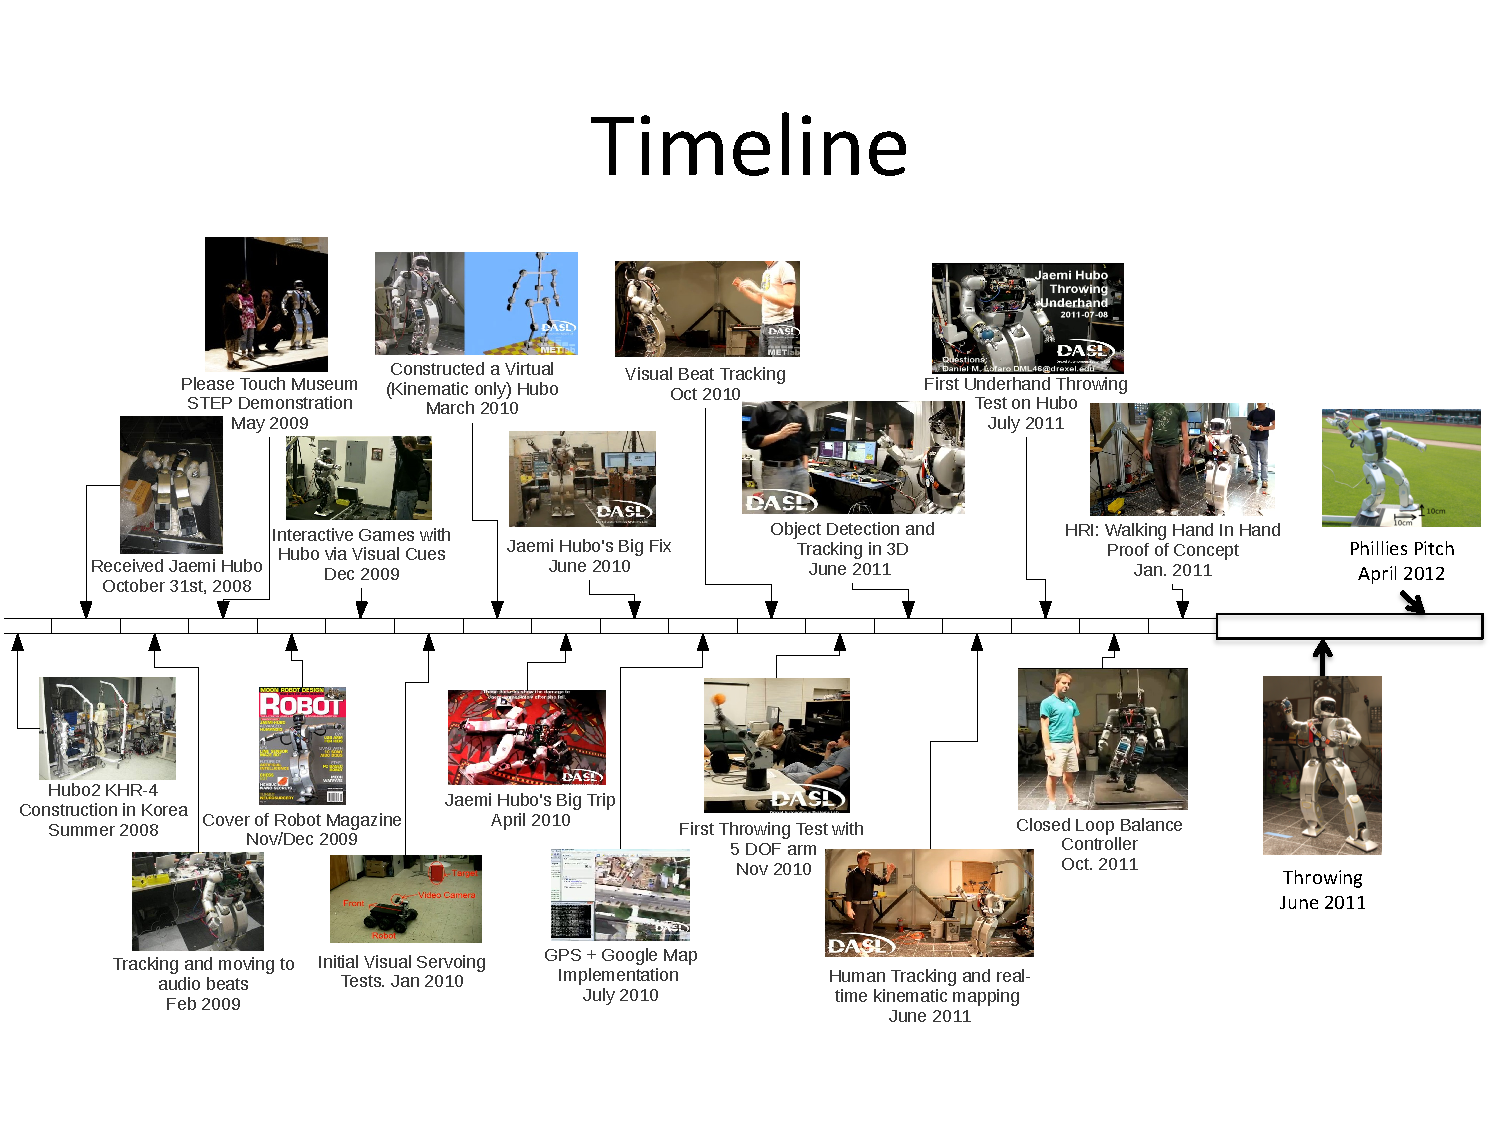
\includegraphics[angle=90, width=0.9\columnwidth]{./pix/Timeline.pdf}
  \caption{Timeline of Daniel M. Lofaro's research from 2008 to 2012}
  \label{fig:timeline}
\end{figure}

Throughout this work Daniel quickly realized that there was no simple and robust way of integrating controllers on top of the existing Hubo control system.
Hubo's original control system was written by Hubo-Lab in the Windows environment utilizing the Real-Time Extension (RTX) for Windows API.
This controller is a typical single loop, single process, real-time controller that gets its high level input via flags and data fields located in shared memory.
As the controller gets more complex it became more and more probable that something would throw a fault.  
If one part of the controller failed the whole system fails.



The Daniel worked with the Drexel Autonomous Systems Lab to create a linux based controller for the Hubo called ACES/Conductor.
This controller designed by Sherbert et. al.\cite{aces} is a multi-threaded real-time controller that breaks each joint into individual devices. 
Each of these devices has multiple layers including the hardware, control, and command layer.
Each of these layers runs their own real-time loop, sharing data via pointer passing for dynamic memory fields.
Though the theoretical concept for this controller was sound, proper implementation would be suitable for an FPGA, GPU or other processors with many cores.
Because each device had multiple real-time loops associated with it (one for each layer) and there are many devices (joints) on the Hubo the CPU usage was high.
When running on a dual core 1.6 Ghz Intel Atom Processor a constant 100\% CPU usage was recorded.
This did not allow other processies to run in tandem.
In addition there was an inherent memory leak in the dynamic memory.
This was brought about from the system never being able to guarantee that another thread is not using a block of memory, thus it is never trashed.
This caused the memory usage to increase at a predictable rate.
This would cause a complete system crash when the memory size surpassed the available memory of the system.
It was found that this system was not suitable to run the Hubo robot.

Learning from the past experiences Daniel sought out to create a controller that could:
\begin{multicols}{2}
\begin{itemize}
\item handel high degrees of freedom
\item simple sensor integration
\item runs in real-time
\item low CPU usage
\end{itemize}
\end{multicols}

This goal was realized with the creation of Hubo-Ach as described in Section~\ref{sec:hubo-ach}. 
Further examples of why Hubo-Ach was created can be found in Appendix~\ref{sec:baseball}